% Chapter 3: Methodology and System Design (full)
% As-built specs (paper): 0.2 m/s, ~2 h runtime, 3-5 min init, MPU6050 IMU, no wheel odometry, ESP32 DevKit, 720p 15 fps, custom frontier + ProxMaP.

\chapter{Methodology and System Design}
\label{ch:method}

\section{Conceptual Framework}
\label{sec:conceptual}

The system utilises a multi-tier autonomous exploration architecture to balance real-time control with the heavy computational demands of AI vision. It is built on three core principles: onboard autonomy for network-independent traversal, multi-level networking (Wi-Fi, 4G, and mesh) with graceful fallback for resilient operator contact, and distributed processing to offload intensive AI tasks to the ground control station. The technological framework integrates ROS~2 \cite{ros2humble} for middleware and sensor fusion, using Google's Cartographer \cite{hess2016} for SLAM to generate 2D occupancy grids. These maps inform the Nav2 stack \cite{nav2dwb} for cost-aware path planning. For communication, the ESP-WiFi-MESH framework \cite{espmesh} enables the UGV to deploy persistent mesh nodes along its path, while 4G hotspot and LoRa provide fallbacks. Finally, an AI perception pipeline on the GCS processes camera feeds to generate actionable mission reports.

\section{High-Level Design}
\label{sec:hld}

Figure~\ref{fig:system_topo} illustrates that the system architecture comprises three primary domains interconnected by a multi-mode communication network. The Unmanned Ground Vehicle (UGV) subsystem combines computing, perception, and locomotion control into a mobile platform that recognises novel surroundings through autonomous navigation. The communication system is constituted by multiple connection modes: ESP-WiFi-MESH as the primary mesh, direct Wi-Fi, 4G cellular, and LoRa at 433\,MHz for resilience and emergency command. All AI perception pipeline, web-based operator dashboard, and mission management interfaces reside at the Ground Control Station (GCS). The two-way data flow allows telemetry and video to be transmitted from the UGV to the GCS, and navigation orders and AI detection results to be sent to the UGV.

% --- FIGURE: System topology ---
\begin{figure}[htbp]
\centering
\includegraphics[width=0.85\textwidth]{figures/system_topology.png}
\caption{System topology and data flow diagram.}
\label{fig:system_topo}
\end{figure}

The operational cycle begins with system initiation (3--5 minutes): the battery system is enabled and the Raspberry Pi~4 boots Ubuntu 22.04 and ROS~2 \cite{ros2humble}. Sensor drivers activate the YDLidar X3 \cite{ydlidar} at 10\,Hz, the MPU6050 IMU, and the cameras at 720p, 15\,fps; the mesh and Wi-Fi/4G links come up. A WebSocket-based web interface at the GCS displays initial diagnostics, including battery voltage, network status, and sensor health. Cartographer SLAM \cite{hess2016} processes LiDAR scans and IMU data (scan-matching and loop closure; no wheel odometry) to generate a 2D occupancy grid. Map updates are transmitted to the GCS for operator monitoring. The Nav2 stack \cite{nav2dwb} uses global and local costmaps for path planning, with the DWB local planner translating velocities into wheel commands. Autonomous exploration is driven by a custom frontier-based method \cite{yamauchi1997} that identifies frontiers, ranks them (including with ProxMaP-style AI map prediction \cite{sharma2022}), and sends goals to Nav2. The cycle continues until coverage is complete or the operator terminates the mission. For perception, video is streamed to the GCS; the operator-side AI runs YOLOv8 detectors and an LLM for scene and hazard analysis, with spatial decision memory (X-SDM) and person profiling. Telemetry is sent at a steady rate. The communication layer switches between mesh, Wi-Fi, and 4G, with LoRa serving as a low-bandwidth fallback for telemetry and return-to-base. The mission concludes when exploration is complete or the battery reaches a safety threshold; the robot can return to base using the recorded map.

\section{Subsystem Design}
\label{sec:subsystem}

\subsection{Power System Design}
\label{sec:power}

The power system provides 24\,V nominal voltage using a modular dual 18650 lithium-ion battery setup. The architecture consists of two 3s3p packs in series, each delivering 11.1\,V nominally (12.6\,V peak), with the series combination giving nominal 22.2--24\,V. Each pack is managed by a BMS providing overvoltage, undervoltage, and overcurrent protection. Usable energy is limited to a safe depth-of-discharge, providing sufficient capacity for almost two hours of continuous operation at 0.2\,m/s in the as-built system. The 24\,V output bifurcates: the high-power branch supplies unregulated voltage to the motor drivers; the low-power branch uses a buck converter to provide a regulated 5\,V rail for the Raspberry Pi~4, sensors (LiDAR, Kinect v1, USB webcam), ESP32-CAM, router, and headlights. The deployable mesh nodes are each powered by a 2500\,mAh LiPo.

% --- FIGURE: Power distribution ---
\begin{figure}[htbp]
\centering
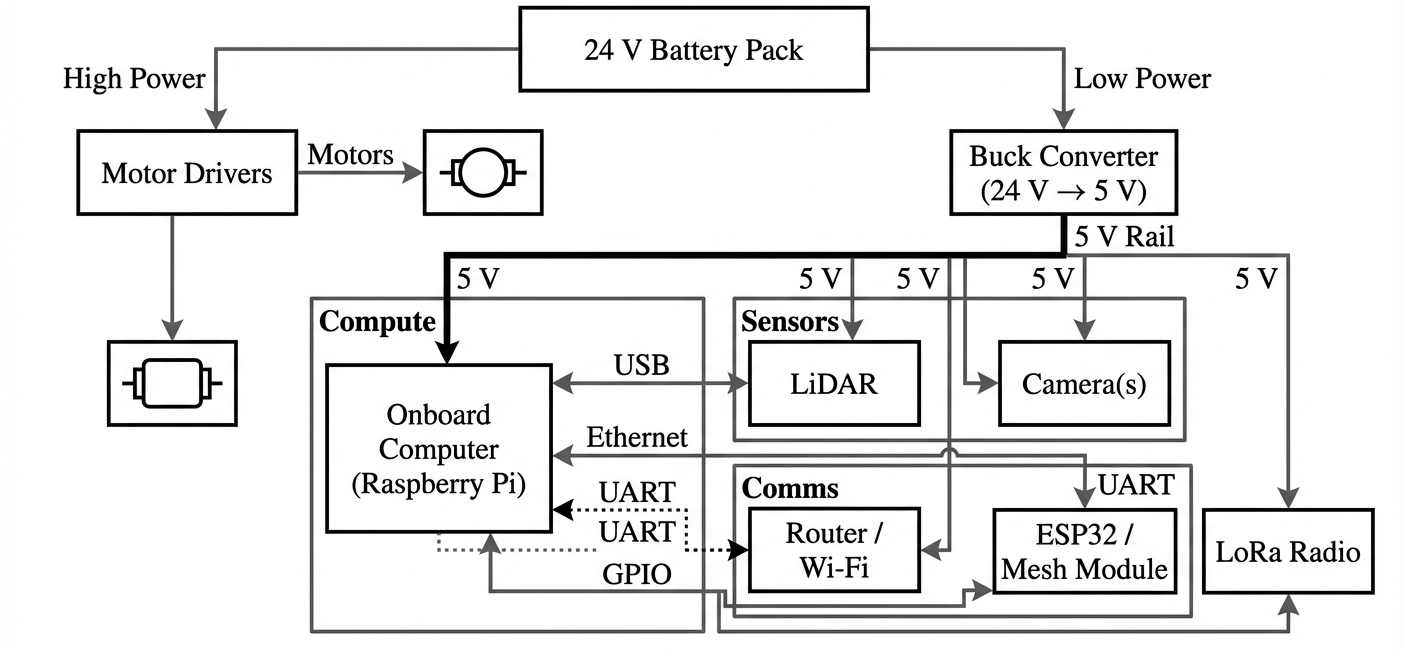
\includegraphics[width=0.7\textwidth]{figures/power_diagram.png}
\caption{Power distribution diagram.}
\label{fig:power_dist}
\end{figure}

\subsection{Locomotion and Control}
\label{sec:locomotion}

The locomotion system uses a 4WD chassis with skid-steering for mobility in cluttered environments. The chassis balances stability and manoeuvrability, allowing passage through standard doorways while maintaining a low centre of gravity. Skid-steering operates on differential-drive principles: left and right wheel pairs are driven independently; forward motion is achieved by matching side speeds, and turning from velocity differences. In-place rotation is possible by counter-rotating the sides. The platform is designed for relatively flat indoor terrain; steep slopes, large rubble, and staircases are outside its operational scope. The system intentionally omits motor encoders, relying solely on Cartographer's scan-matching for localisation. This reduces hardware complexity and cost. To keep scan-matching reliable, autonomous speed is capped at 0.2\,m/s; at 10\,Hz LiDAR, the robot travels 20\,mm between scans, ensuring strong feature overlap. Locomotion is optimised for partially intact indoor buildings, with the ability to clear minor obstacles such as doorsteps or cables. The control architecture uses an ESP32 (or equivalent) as an intermediary between the Raspberry Pi~4 and the motor drivers where appropriate; velocity commands from Nav2 are published to \texttt{/cmd\_vel} and converted to motor outputs.

% --- FIGURE: Chassis dimensions ---
\begin{figure}[htbp]
\centering
\includegraphics[width=0.6\textwidth]{figures/chassis_dimensions.png}
\caption{Planned dimensions of the UGV chassis.}
\label{fig:chassis}
\end{figure}

The motor driver and configuration are shown in Figure~\ref{fig:motor_config}.
\begin{figure}[htbp]
\centering
\includegraphics[width=0.6\textwidth]{figures/motor_config.png}
\caption{Motor configuration and drive interface.}
\label{fig:motor_config}
\end{figure}

\subsection{Perception and Mapping}
\label{sec:perception_mapping}

The perception and mapping subsystem provides real-time localisation and map generation. The system uses a YDLidar X3 2D laser scanner: 360° range 0.12--12\,m, 10\,Hz scan rate, approximately 1° angular resolution. It connects to the Raspberry Pi~4 via USB--UART. A Microsoft Kinect v1 is used as an RGB-D camera under budget constraints; its point cloud is fused into the Nav2 local costmap to improve obstacle avoidance for overhangs and table legs. Vision for the operator is provided by a USB webcam (main) and an ESP32-CAM (rear), both at 720p and 15\,fps \cite{ydlidar}.

Google Cartographer serves as the SLAM framework, using graph-based optimisation to estimate robot poses and create 2D occupancy grids \cite{hess2016}. The algorithm maintains a pose graph; when the robot returns to a previously visited area, Cartographer performs loop closure to eliminate cumulative drift. Cartographer was selected for its robust approach, allowing accurate positioning from LiDAR data and the MPU6050 IMU, without requiring wheel encoders. The framework uses a hierarchical submap approach; real-time scans are matched against submaps to build the grid. The system uses an occupancy grid resolution of 0.05\,m (5\,cm). The software platform is Ubuntu 22.04 LTS running ROS~2 Humble \cite{ros2humble}. The Raspberry Pi~4 (8\,GB RAM) provides the necessary processing for Cartographer at 10\,Hz. The coordinate frame architecture follows ROS~2 conventions: the map--odom--base\_link--laser\_link transform chain; Cartographer publishes map$\to$odom to correct drift. The laser frame is set with a static offset from base\_link for accurate spatial projection. Loop closure reduces drift to under approximately 5\,cm in feature-rich regions; in feature-poor areas drift can reach approximately 20--30\,cm until a distinctive feature is revisited. Figure~\ref{fig:carto_posegraph} shows the Cartographer pose graph and loop closure; the TF coordinate frame tree is illustrated in Figure~\ref{fig:tf_tree}. Limitations include inability to detect obstacles outside the LiDAR plane (e.g.\ overhanging cables) and sensitivity to glass; these are accepted for floor-level reconnaissance.

% --- FIGURE: Cartographer pose graph ---
\begin{figure}[htbp]
\centering
\includegraphics[width=0.75\textwidth]{figures/carto_posegraph.jpg}
\caption{Cartographer pose graph and loop closure.}
\label{fig:carto_posegraph}
\end{figure}

\begin{figure}[htbp]
\centering
\includegraphics[width=0.7\textwidth]{figures/tf_tree.jpg}
\caption{TF coordinate frame tree (map, odom, base\_link, laser).}
\label{fig:tf_tree}
\end{figure}

% --- FIGURE: Occupancy grid ---
\begin{figure}[htbp]
\centering
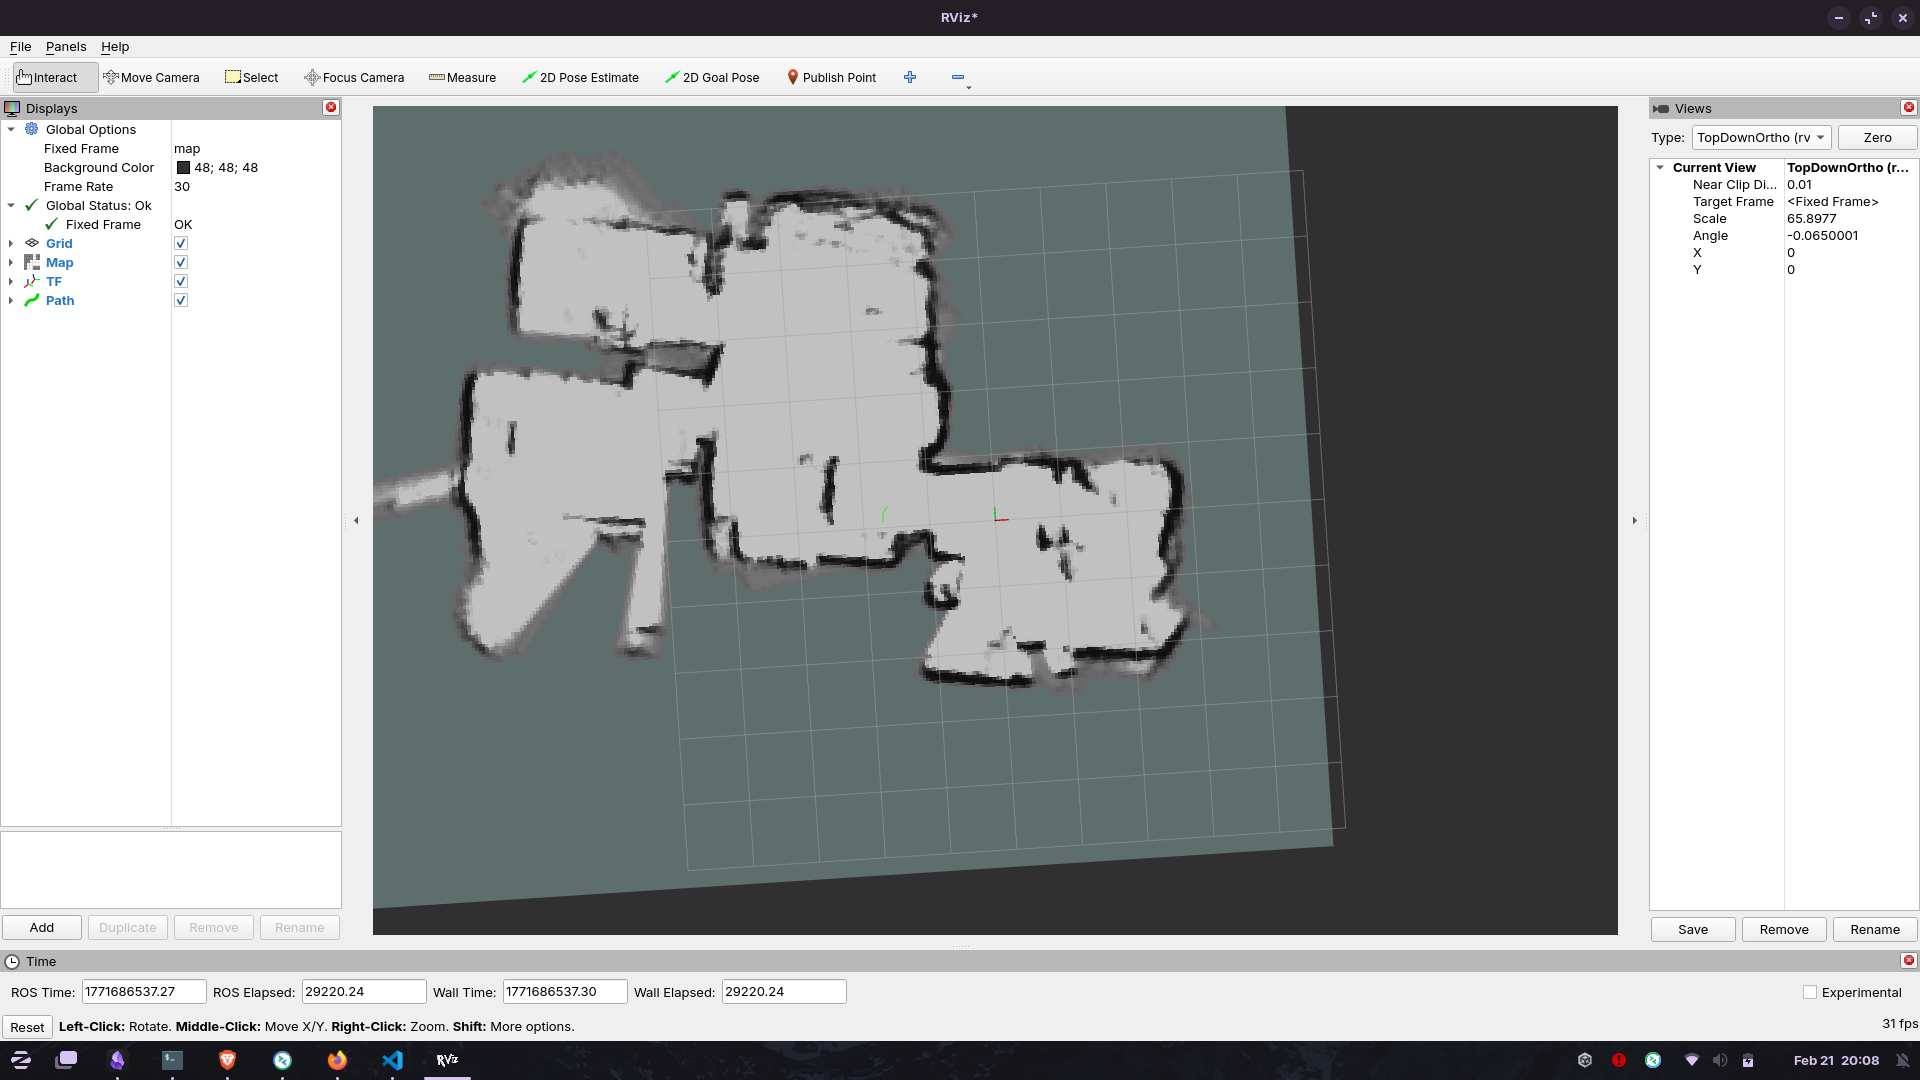
\includegraphics[width=0.75\textwidth]{figures/occupancy_grid.png}
\caption{Occupancy grid generated by SLAM.}
\label{fig:occupancy_grid}
\end{figure}

\subsection{Navigation and Autonomous Exploration}
\label{sec:nav_explore}

The navigation and autonomous exploration subsystem converts SLAM occupancy grids into robot motion. The system uses the ROS~2 Navigation Stack (Nav2): global path planning, local trajectory optimisation (DWB controller), and costmap management. Nav2 processes the Cartographer grid and pose to compute collision-free paths and publishes velocity commands to \texttt{/cmd\_vel}. The global planner uses Dijkstra's algorithm on the occupancy grid \cite{rachmawati2020}; the local planner uses the Dynamic Window Approach (DWB) \cite{nav2dwb} for obstacle avoidance and smooth trajectories \cite{gomez2024}. Costmaps combine a static layer from SLAM, an obstacle layer (LiDAR and Kinect v1 point cloud in the local costmap), and an inflation layer (0.3\,m safety margin). The global costmap uses the full grid and updates at a moderate rate; the local costmap maintains a rolling window around the robot for real-time obstacle reaction. Figure~\ref{fig:nav2_costmap} shows the Nav2 local costmap and obstacle layer.

\begin{figure}[htbp]
\centering
\includegraphics[width=0.8\textwidth]{figures/nav2_costmap.png}
\caption{Nav2 local costmap and obstacle layer.}
\label{fig:nav2_costmap}
\end{figure}

Autonomous exploration is handled by a custom-built frontier-based package that integrates with Nav2 \cite{yamauchi1997}. Frontier cells are free cells with at least one unknown neighbour (a 5$\times$5 window handles Cartographer's border). Frontiers are clustered with 8-connected BFS and scored using a linear combination of spatial and heuristic factors:
\begin{equation}
Score(f_i) = \alpha \cdot G(f_i) + \beta \cdot H(f_i) + \gamma \cdot I_{AI}(f_i) - \delta \cdot D(x_r, f_i)
\label{eq:frontier_score}
\end{equation}
where $G(f_i)$ is the grid cluster size of the $i$-th frontier, $H(f_i)$ is the heading bonus prioritising forward-facing exploration, $I_{AI}(f_i)$ is the AI map-prediction information gain, $D(x_r, f_i)$ is the Dijkstra path distance from the current robot pose $x_r$, and the Greek letters represent empirically tuned constraint weights. Figure~\ref{fig:detected_frontiers} shows detected frontier cells and clustering. The AI map-prediction layer defining $I_{AI}(f_i)$ runs a ProxMaP U-Net \cite{sharma2022} on a $128\times128$ robot-centred map crop. The network accepts a two-channel input (normalised occupancy and an unknown-cell mask) and outputs three-class logits (free, occupied, unknown). It was trained self-supervised on approximately 6\,000 map pairs from the AI2THOR simulator \cite{sharma2022}, achieving 85.43\% prediction accuracy and an F1 score of 87.42\% on the occupied class. In the original study, the predictor improved navigation efficiency by 12.4\% (SCT metric) over a non-predictive baseline. In our system the predicted map boosts the score of frontiers bound for open space, effectively reducing backtracking. The explorer supports dynamic replanning and manual no-go zones via RViz. Recovery behaviours include rotate-in-place, back-up, and costmap clearing. Exploration terminates when no frontiers remain, when battery reaches a configurable minimum (return-to-base), or when the operator aborts. Teleoperation override is supported: control inputs from the GCS override autonomous commands; when manual input ceases, the system resumes exploration.

% --- FIGURE: Detected frontiers ---
\begin{figure}[htbp]
\centering
\includegraphics[width=0.75\textwidth]{figures/detected_frontiers.jpg}
\caption{Detected frontier cells and clustering.}
\label{fig:detected_frontiers}
\end{figure}

The global planner computes shortest paths on the occupancy grid using Dijkstra's algorithm; the path is computed on the discrete grid and then followed by the local planner. When an obstacle appears in the planned path (for example when the LiDAR or Kinect detects a new obstacle), the costmap is updated and the path is recomputed. Figure~\ref{fig:nav_paths} shows a typical Dijkstra path and the path before and after obstacle replanning.

\begin{figure}[t]
\centering
\includegraphics[width=0.72\textwidth]{figures/dijkstra_path.jpg}\\[6pt]
\begin{minipage}[t]{0.48\textwidth}
\centering
\includegraphics[width=\linewidth]{figures/path_before_obstacle.png}\\
(a) Before obstacle detection
\end{minipage}\hfill
\begin{minipage}[t]{0.48\textwidth}
\centering
\includegraphics[width=\linewidth]{figures/path_after_obstacle.png}\\
(b) After replanning
\end{minipage}
\caption{Navigation path planning: Dijkstra pathfinding (top); path before and after obstacle detection (bottom).}
\label{fig:nav_paths}
\end{figure}

The local planner (DWB) tracks the global path while avoiding obstacles. Once the obstacle is incorporated into the local costmap, Nav2 replans and the robot follows an updated path that avoids the obstacle. This behaviour ensures that exploration continues safely even when the environment changes during a run.

\clearpage
\subsection{Communication and Network Architecture}
\label{sec:comms_design}

The communication subsystem offers robust connectivity between the UGV and GCS. The architecture uses four redundant technologies: ESP-WiFi-MESH \cite{espmesh} for extended multi-hop routing, direct Wi-Fi for high-bandwidth local transfer, 4G cellular when Wi-Fi is out of range, and 433\,MHz LoRa (SX1278) as a low-bandwidth emergency backup. These modes are managed so that high-performance links are preferred while lower-bandwidth channels remain as fallbacks.

Rather than treating each outage independently, the design follows an ordered degradation policy. The active tier advances from Wi-Fi (full video, map, and control traffic) to 4G when the local Wi-Fi path fails sustained health checks, then to ESP mesh with compressed imagery and reduced map update rates, and finally to LoRa for essential telemetry and safety-related commands when no IP backhaul is available. Downgrades use relatively short timeouts so the operator is not left on a dead link; recovery to a higher tier is gated by longer stable-good intervals (hysteresis) to avoid oscillation at building boundaries. Figure~\ref{fig:state_diagram} summarises this state-oriented view alongside the physical topology in Figure~\ref{fig:network_topo}.

\begin{figure}[htbp]
\centering
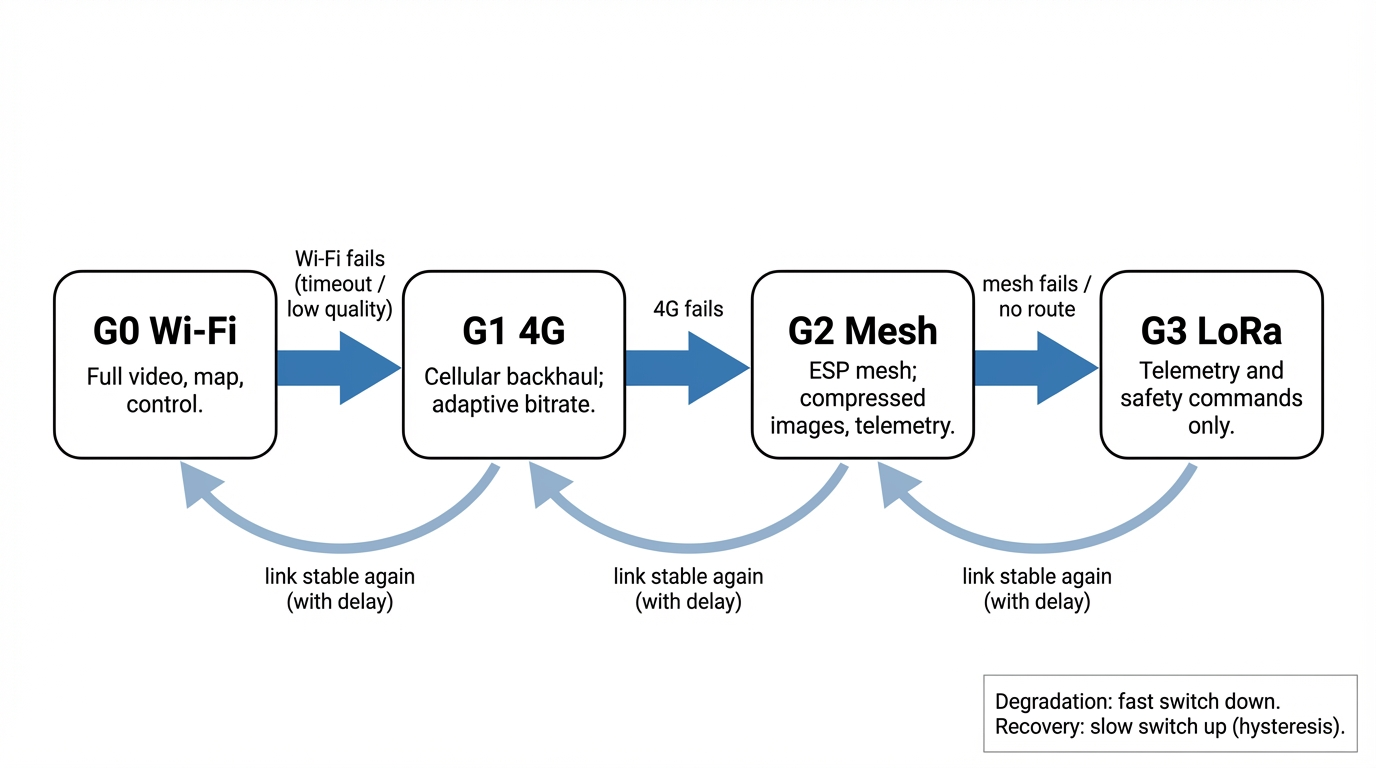
\includegraphics[width=0.92\textwidth]{figures/state_diagram.jpeg}
\caption{Network degradation state machine: preferred progression Wi-Fi $\rightarrow$ 4G $\rightarrow$ mesh $\rightarrow$ LoRa, with slower upgrade paths to limit link flapping.}
\label{fig:state_diagram}
\end{figure}

The backbone uses ESP-WiFi-MESH on ESP32 DevKit microcontrollers \cite{espmesh}. The UGV deploys up to two nodes along its path via a servo mechanism. To ensure a resilient connection pipeline without saturating the environment, the autonomous deployment trigger is dictated by a threshold function evaluating wireless link quality constraints:
\begin{equation}
D_{trigger} = 
\begin{cases} 
1, & \textbf{if } \text{RSSI}_{avg}(t) < -80\,\text{dBm} \text{ for } \Delta t \ge 3\,\text{s} \\
1, & \textbf{if } \text{PDR} < 85\% \\
0, & \textbf{otherwise}
\end{cases}
\label{eq:mesh_deployment}
\end{equation}
where $\text{RSSI}_{avg}$ is the moving average of the received signal strength indicator and $\text{PDR}$ is the real-time packet delivery ratio. Once triggered ($D_{trigger} = 1$), the node is released and automatically added to the active routing table. Nodes are powered by a 2500\,mAh LiPo each. When only mesh is available, images are iteratively WebP-compressed to a strict 8\,kB limit, Base64-encoded, and reconstructed at the operator side. Direct Wi-Fi (e.g.\ TP-Link Archer C6 on UGV, Tenda F3 at GCS) provides high bandwidth when the UGV is within range; throughput drops with walls and distance. The 4G hotspot provides wide-area connectivity when Wi-Fi is unavailable. The LoRa SX1278 link carries critical telemetry (position, battery, status) and emergency commands (e.g.\ return-to-base) when other links fail. The multi-tier design ensures graceful degradation from real-time video to periodic images to text-only telemetry.

% --- FIGURE: Network topology ---
\begin{figure}[htbp]
\centering
\includegraphics[width=0.8\textwidth]{figures/network_topology.jpg}
\caption{Network topology diagram.}
\label{fig:network_topo}
\end{figure}

\subsection{Vision and AI Perception}
\label{sec:vision_ai}

The vision and AI perception subsystem includes real-time object detection, LLM-based scene understanding, spatial decision memory (X-SDM), and mission logging. The visual system uses a USB webcam (main) and an ESP32-CAM (rear), both at 720p and 15\,fps. Video is streamed over the main link when Wi-Fi or 4G is available; on link degradation, images are sent over the mesh. AI perception is offloaded to the operator workstation to preserve the UGV's power budget and to leverage GPUs for fast inference.

The detection pipeline runs three YOLOv8m \cite{jocher2023yolov8} models (25.9M parameters each) in parallel: a fire/smoke detector fine-tuned on the Kerby Fire/Smoke dataset \cite{kerby2024firesmoke} (approximately 11\,000 images, two classes), a human detector using the default COCO pre-trained person class (class~0), and an extinguisher detector fine-tuned on the Roboflow FireExtinguisher dataset \cite{fireextinguisher2022roboflow} (3\,300 images, eight classes). Confidence thresholds are set to 0.45, 0.35, and 0.30 for fire, human, and extinguisher respectively; cross-model outputs are merged with non-maximum suppression at an IoU threshold of 0.7. Contextual reasoning is handled by an LLM (Llama-4-Scout via Groq), which processes YOLO outputs and SLAM context to generate mission intelligence. The Explainable Spatial Decision Memory (X-SDM) layer merges semantic LLM scene-matching with deterministic SLAM geometry to classify environments. For a given current frame and a candidate historical location, the decision $X_{decision}$ evaluates to either a \texttt{REVISIT} or \texttt{NEW\_LOCATION}:
\begin{equation}
X_{decision} = 
\begin{cases} 
\text{\texttt{REVISIT}}, & \text{if } M_{LLM} = \text{True} \text{ and } C_{LLM} \ge \tau_{XSDM} \\
\text{\texttt{REVISIT}}, & \text{if } M_{LLM} = \text{False} \text{ and } d_{SLAM} < d_{micro} \text{ and } C_{LLM} \ge 0.5 \\
\text{\texttt{NEW\_LOCATION}}, & \text{otherwise}
\end{cases}
\label{eq:xsdm_decision}
\end{equation}
where $M_{LLM}$ is the boolean topological match predicted by the LLM based on visual landmarks, $C_{LLM} \in [0, 1]$ is the self-reported confidence of that semantic match, and $\tau_{XSDM}$ (empirically set to $0.65$) is the system acceptance threshold. To prevent hallucinating duplicate rooms when physically stationary, the secondary logical branch overrides the LLM and forces a revisit if the robot's Euclidean displacement $d_{SLAM}$ from the candidate is less than a rigid spatial anchor $d_{micro}$ (e.g., $0.3$\,m). Parallel to this, dynamic person profiling employs code-level deduplication; the pipeline generates a descriptive visual profile (clothing, build, posture) for every human detected and assigns a unique identification string. If a subsequent algorithmic evaluation matches a new person to an existing profile, it updates the status without emitting redundant map annotations. When a genuinely novel hazard or person annotation is needed, markers (e.g.\ sphere and label at map coordinates, severity-coloured) are published to a ROS~2 topic and the dashboard draws them. Mission data is logged to JSONL and CSV for post-mission analysis.

% --- FIGURE: Perception pipeline ---
\begin{figure}[htbp]
\centering
\includegraphics[width=0.8\textwidth]{figures/perception_pipeline.jpg}
\caption{Complete vision and AI perception pipeline.}
\label{fig:perception_pipeline}
\end{figure}

\subsection{Ground Control Station}
\label{sec:gcs_design}

The Ground Control Station (GCS) provides the human--machine interface for mission supervision and manual override. It uses a web architecture: a frontend (e.g.\ JavaScript/React) and a FastAPI \cite{fastapi} backend. The dashboard interacts with the robot's ROS~2 environment through rosbridge \cite{rosbridge}, translating topics into messages for the browser. Key streams include the occupancy map, robot pose, and AI detections. Commands such as \texttt{/cmd\_vel} for teleoperation and exploration goals are sent over the same bidirectional link. The mapping panel renders the occupancy grid with robot pose and AI annotations (e.g.\ hazards, persons) as severity-coded icons. The video feed toggles between streaming (Wi-Fi/4G) and highly-compressed WebP snapshots reconstructed via AI (mesh). The dashboard shows battery voltage, signal strength across links, and mission elapsed time. An AI detection feed provides chronological logs (YOLO labels, LLM reasoning, X-SDM). Operators can switch between autonomous and manual modes; in manual mode, a virtual joystick or keyboard sends velocity commands. High-level buttons (Start, Pause, Return to Base, Emergency Stop) and natural-language summaries provide a mission narrative. See Chapter~\ref{ch:impl} for the as-built operator dashboard implementation.

% --- FIGURE: X-SDM flowchart ---
\begin{figure}[htbp]
\centering
\includegraphics[width=0.65\textwidth]{figures/xsdm_flowchart.jpg}
\caption{X-SDM decision tree/flowchart.}
\label{fig:xsdm}
\end{figure}

\clearpage
